%!TEX TS-program = xelatex
\documentclass[en]{hust-thesis} % use [vi] for vietnamese

\usepackage{blindtext}

\title{This is title of the thesis}
\author{Bui Hong Ngoc}
\authoremail{myemail@sis.hust.edu.vn}
\major{Computer Science}
\field{Information Technology}
\advisor{Prof. Do Phan Thuan}
\department{Department of Computer Science}
\institute{School of Information and Communication Technology}
\degree{Thesis}
\university{Hanoi University of Science and Technology}
\universitycity{Hanoi}
\universitystate{Hanoi}
\degreemonth{5}
\degreeyear{2021}

\renewcommand{\glsmcols}{1}
\setglossarystyle{list}

\newacronym{gec}{GEC}{Grammatical Error Correction}
\newacronym{esl}{ESL}{English as a Second Language}
\newacronym{rl}{RL}{Reinforcement Learning}
\newacronym{dl}{DL}{Deep Learning}
\newacronym{ml}{ML}{Machine Learning}
\newacronym{nlp}{NLP}{Natural Language Processing}
\newacronym{bert}{BERT}{Bidirectional Encoder Representations from Transformers}
\newacronym{gpu}{GPU}{Graphics Processing Unit}
\newacronym{s2s}{seq2seq}{Sequence-to-Sequence}

\newglossary[nlg]{notation}{not}{ntn}{Notation}

\newglossaryentry{not:eth}{
  name=\ensuremath{\tilde{E}_{td}},
  description={energy requesting threshold},
  type=notation}

\newglossaryentry{not:bs}{
  name=\ensuremath{p_0},
  description={base station},
  type=notation}

\newglossaryentry{not:snset}{
  name=\ensuremath{\mathcal{P}},
  description={a set of deployed sensors},
  type=notation}

\newglossaryentry{not:num:sn}{
  name=\ensuremath{n},
  description={number of deployed sensors},
  type=notation}

\newglossaryentry{not:sn}{
  name=\ensuremath{p},
  description={a sensor},
  type=notation}


\makeglossaries 

\begin{document}

%%%%%%%%%%%%%%%%%%%%%%%%%%%%%%%%
%title
%%%%%%%%%%%%%%%%%%%%%%%%%%%%%%%%
\maketitle
%

\copyrightpage

\authorphone{0383090063}
\authorclass{CTTT Điện tử 01-K64}
\duration{01/09/2024 - 03/02/2025}

\statement{
  This thesis focuses on the development of a web-based application that provides easy access to existing grammatical error correction (GEC) models using advanced natural language processing (NLP) techniques.
  It does not introduce a new GEC method nor improve the performance of existing models.
  Instead, the goal is to make state-of-the-art GEC technology more accessible and user-friendly for the general public by integrating these models into an intuitive and lightweight web interface.
}

\declaration{
  I hereby declare that this thesis is my original work and has not been submitted for any degree or diploma at any other institution.
  Any materials or ideas derived from other sources have been properly cited.
  Furthermore, I declare that there are no conflicts of interest affecting this research.
  % All information cited complies with the intellectual property regulations.
  % The references are clearly listed.
  % I take full responsibility for the content written in this thesis.
}

\requirementpage

\pagenumbering{roman}

\acknowledgments{
Lorem ipsum dolor sit amet, consetetur sadipscing elitr, sed diam nonumy eirmod tempor invidunt ut labore et dolore magna aliquyam erat, sed diam voluptua. At vero eos et accusam et justo duo dolores et ea rebum. Stet clita kasd gubergren, no sea takimata sanctus est Lorem ipsum dolor sit amet. 

Lorem ipsum dolor sit amet, consetetur sadipscing elitr, sed diam nonumy eirmod tempor invidunt ut labore et dolore magna aliquyam erat, sed diam voluptua. At vero eos et accusam et justo duo dolores et ea rebum. Stet clita kasd gubergren, no sea takimata sanctus est Lorem ipsum dolor sit amet. 

Lorem ipsum dolor sit amet, consetetur sadipscing elitr, sed diam nonumy eirmod tempor invidunt ut labore et dolore magna aliquyam erat, sed diam voluptua. At vero eos et accusam et justo duo dolores et ea rebum. Stet clita kasd gubergren, no sea takimata sanctus est Lorem ipsum dolor sit amet.

Duis autem vel eum iriure dolor in hendrerit in vulputate velit esse molestie consequat, vel illum dolore eu feugiat nulla facilisis at vero eros et accumsan et iusto odio dignissim qui blandit praesent luptatum zzril delenit augue duis dolore te feugait nulla facilisi. Lorem ipsum dolor sit amet, consectetuer adipiscing elit, sed diam nonummy nibh euismod tincidunt ut laoreet dolore magna aliquam erat volutpat.}

\addcontentsline{toc}{chapter}{Abstract}
\abstractpage{
  This thesis presents a lightweight web application to serve grammatical error correction (from now on refers as GecWeb) systems so that they can be easily used by the general public.
  I design GecWeb to be accessible to as many users as possible, including users who have a slow Internet connection and who use mobile phones as their main devices to connect to the Internet.
  GecWeb provides three state-of-the-art base GEC systems using sequence tagging, as well as two state-of-the-art GEC system combination methods using two approaches (edit-based and text-based).

  % It is suggested to have the abstract in both language (Vietnamese and English).
  \newpage
  \begin{center}
    \vspace*{1pt}
    \Large \textcolor{Crimson}{\textit{Ứng dụng sửa lỗi ngữ pháp sử dụng học máy}} \normalsize\\
    \vspace*{15pt}
    {\bf Tóm tắt đồ án} \rm
  \end{center}

  Luận văn này trình bày một ứng dụng web nhẹ để phục vụ chỉnh sửa lỗi ngữ pháp (sau đây gọi là GecWeb), giúp công chúng dễ dàng tiếp cận và sử dụng.
  GecWeb được thiết kế nhằm đảm bảo khả năng tiếp cận rộng rãi nhất có thể, bao gồm cả những người dùng có kết nối Internet chậm và những người sử dụng điện thoại di động làm thiết bị chính để truy cập Internet.
  GecWeb cung cấp ba hệ thống chỉnh sửa lỗi ngữ pháp (GEC) tiên tiến sử dụng phương pháp gán nhãn chuỗi (sequence tagging), cũng như hai phương pháp kết hợp hệ thống GEC hiện đại dựa trên hai cách tiếp cận khác nhau (dựa trên chỉnh sửa và dựa trên văn bản).
}


\tableofcontents
\addcontentsline{toc}{chapter}{List of Figures}
\listoffigures
\addcontentsline{toc}{chapter}{List of Tables}
\listoftables

\glsaddall
\printglossary[type=\acronymtype,title=List of Acronyms, toctitle=List of Acronyms]
\printglossary[type=notation,title=List of Notations, toctitle=List of Notations,nonumberlist]

\newpage
\pagenumbering{arabic}


\begin{savequote}[75mm] 
Nulla facilisi. In vel sem. Morbi id urna in diam dignissim feugiat. Proin molestie tortor eu velit. Aliquam erat volutpat. Nullam ultrices, diam tempus vulputate egestas, eros pede varius leo.
\qauthor{Quoteauthor Lastname} 
\end{savequote}

\chapter{The title of chapter one}

\newthought{There's something to be said} for having a good opening line. Morbi commodo, ipsum sed pharetra gravida, orci  $x = 1/\alpha$ magna rhoncus neque, id pulvinar odio lorem non turpis \citep{Eigen1971, Knuth1968}. Nullam sit amet enim. Suspendisse id velit vitae ligula volutpat condimentum. Aliquam erat volutpat. Sed quis velit. Nulla facilisi. Nulla libero. Vivamus pharetra posuere sapien. Nam consectetuer. Sed aliquam, nunc eget euismod ullamcorper, lectus nunc ullamcorper orci, fermentum bibendum enim nibh eget ipsum. Donec porttitor ligula eu dolor. Maecenas vitae nulla consequat libero cursus venenatis. Nam magna enim, accumsan eu, blandit sed, blandit a, eros.
$$\zeta = \frac{1039}{\pi}$$


For an example of a full page figure, see Fig.~\ref{fig:myFullPageFigure}.

\section{This is section one}

\blindtext


\blindtext


\begin{figure}  
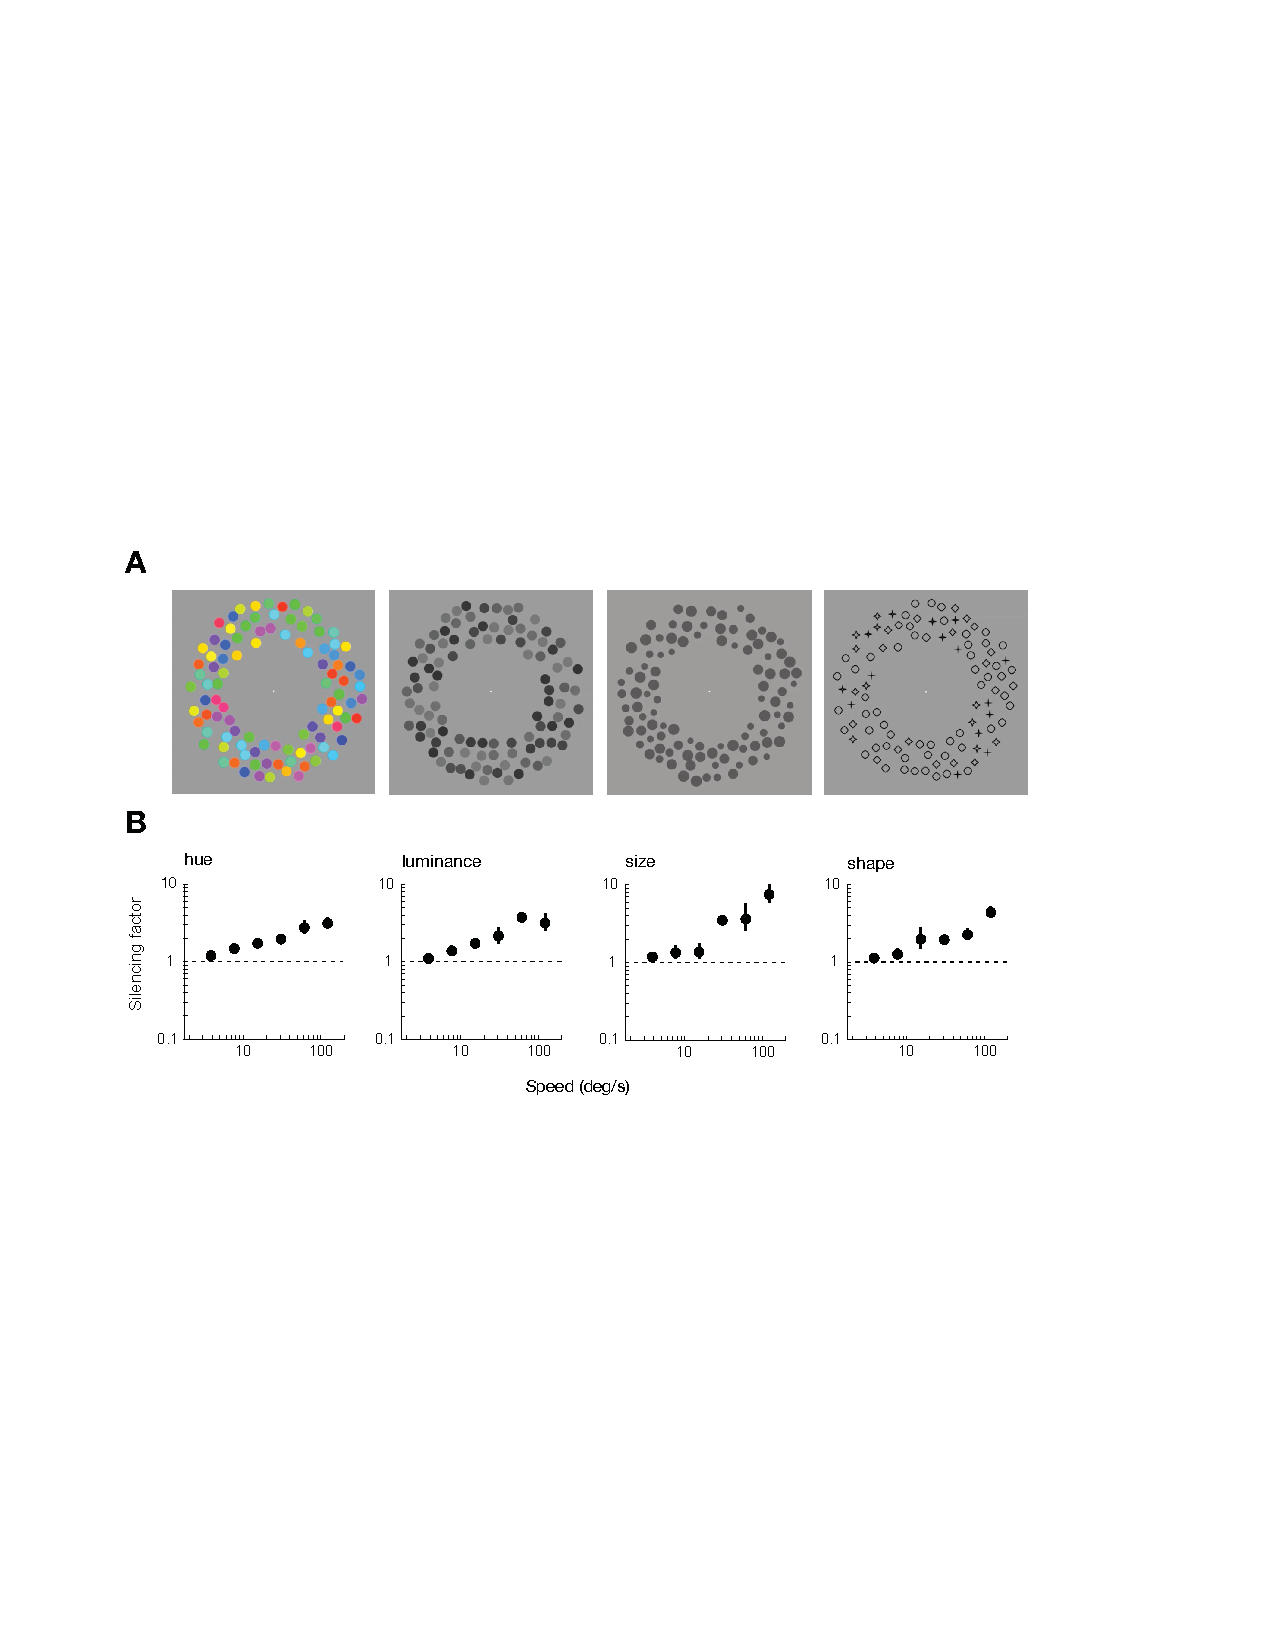
\includegraphics[width=\textwidth]{figures/fig1}
\caption[Short figure name.]{This is a figure that floats inline and here is its caption.
\label{fig:myInlineFigure}}
\end{figure}

\blindtext

\begin{figure}  
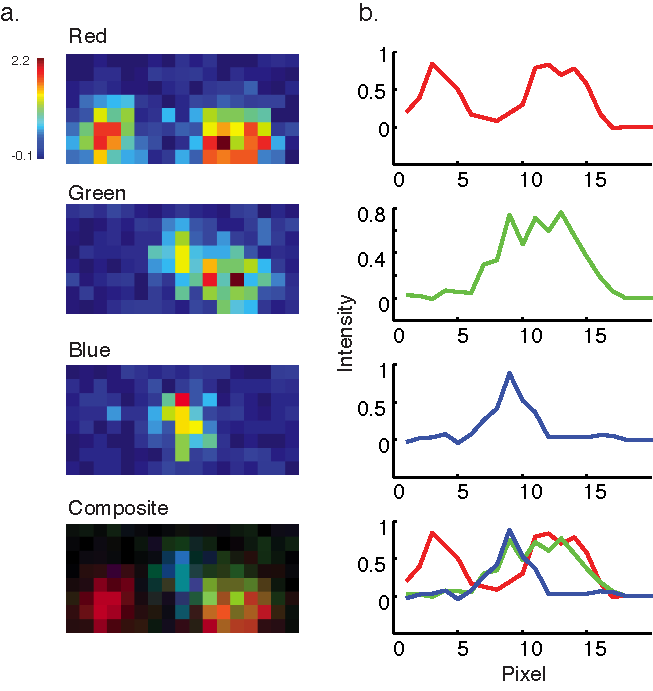
\includegraphics[width=\textwidth]{figures/fullpage}
\caption[Short figure name.]{This is a full page figure using the FPfigure command. It takes up the whole page and the caption appears on the preceding page. Its useful for large figures. Harvard's rules about full page figures are tricky, but you don't have to worry about it because we took care of it for you. For example, the full figure is supposed to have a title in the same style as the caption but without the actual caption. The caption is supposed to appear alone on the preceding page with no other text. You do't have to worry about any of that. We have modified the fltpage package to make it work. This is a lengthy caption and it clearly would not fit on the same page as the figure. Note that you should only use the FPfigure command in instances where the figure really is too large. If the figure is small enough to fit by the caption than it does not produce the desired effect. Good luck with your thesis. I have to keep writing this to make the caption really long. LaTex is a lot of fun. You will enjoy working with it. Good luck on your post doctoral life! I am looking forward to mine. \label{fig:myFullPageFigure}}
\end{figure}
\afterpage{\clearpage}

\blindtext

\section{This is section two}
\blindtext
\blindmathpaper

\section{This is section three}
\blindtext
\blindmathpaper
\begin{savequote}[75mm] 
This is some random quote to start off the chapter.
\qauthor{Firstname lastname} 
\end{savequote}

\chapter{The title of chapter two}

\newthought{Lorem ipsum dolor sit amet}, consectetuer adipiscing elit. Morbi commodo, ipsum sed pharetra gravida, orci magna rhoncus neque, id pulvinar odio lorem non turpis. Nullam sit amet enim. Suspendisse id velit vitae ligula volutpat condimentum. Aliquam erat volutpat. Sed quis velit. Nulla facilisi. Nulla libero. Vivamus pharetra posuere sapien. Nam consectetuer. Sed aliquam, nunc eget euismod ullamcorper, lectus nunc ullamcorper orci, fermentum bibendum enim nibh eget ipsum. Donec porttitor ligula eu dolor. Maecenas vitae nulla consequat libero cursus venenatis. Nam magna enim, accumsan eu, blandit sed, blandit a, eros.

\section{This is section one}
\blindtext

\blinditemize

\begin{table}[tb]
  \centering
  \caption{Network constants of the energy model.}
  \label{tab:network_constants}
  \small
  % \begin{tabular*}{\textwidth}{l @{\extracolsep{\fill}} l}
  \begin{tabular}{lll}
    \toprule
    Parameter & Value & Unit \\
    \midrule
    $\epsilon_{elec}$ & $50$ &  $nJ/bit$ \\
    $\epsilon_{fs}$ & $10$ & $pJ/bit/m^2$ \\
    $\epsilon_{mp}$ & $0.0013$ & $pJ/bit/m^4$ \\
    \bottomrule
  \end{tabular}
  % \end{tabular*}
\end{table} 


\blindmathpaper

\blindtext@formula 

\section{This is section two}
\blindtext
\blindmathpaper

\section{This is section three}
\blindtext
\blindmathpaper
\begin{savequote}[75mm] 
Nulla facilisi. In vel sem. Morbi id urna in diam dignissim feugiat. Proin molestie tortor eu velit. Aliquam erat volutpat. Nullam ultrices, diam tempus vulputate egestas, eros pede varius leo.
\qauthor{Quoteauthor Lastname} 
\end{savequote}

\chapter{Consectetuer adipiscing elit}

\newthought{Lorem ipsum dolor sit amet}, consectetuer adipiscing elit. Morbi commodo, ipsum sed pharetra gravida, orci magna rhoncus neque, id pulvinar odio lorem non turpis. Nullam sit amet enim. Suspendisse id velit vitae ligula volutpat condimentum. Aliquam erat volutpat. Sed quis velit. Nulla facilisi. Nulla libero. Vivamus pharetra posuere sapien. Nam consectetuer. Sed aliquam, nunc eget euismod ullamcorper, lectus nunc ullamcorper orci, fermentum bibendum enim nibh eget ipsum. Donec porttitor ligula eu dolor. Maecenas vitae nulla consequat libero cursus venenatis. Nam magna enim, accumsan eu, blandit sed, blandit a, eros.

\blindtext

\section{This is section one}
\blindtext
\blindmathpaper

\section{This is section two}
\blindtext
\blindmathpaper

\clearpage
\bibliography{refs}
\addcontentsline{toc}{chapter}{References}
\bibliographystyle{plainnat}

\begin{appendices}
\chapter{This is title of appendix A}
\blindmathpaper
\chapter{This is title of appendix B}
\blindmathpaper
\end{appendices}

\end{document}
